\documentclass[12pt]{article}
\usepackage{graphicx}
\addtolength{\evensidemargin}{-0.5in}
\addtolength{\oddsidemargin}{-0.5in}
\addtolength{\textwidth}{1.0in}
\begin{document}
\begin{center}
{\large\bf A Monte Carlo Model of Electromagnetic Showers
}
\end{center}
\vspace{0.2cm}
In order to understand how their detectors respond, physicists
use complex simulations.  These simulations take as their input Monte Carlo
generated events, propagate the particles in these events through a model
of the detector and simulate the response.  The output of the simulation
is written in the same format as the real data and is used
to understand the experiment's ``acceptance'' and resolution.
Proper modeling of the detector response requires detailed understanding
of the physics of particle interactions with matter.  Today, most
experiments use a simulation toolkit, called Geant4, to model this physics.
In this problem, you will write your own Monte Carlo simulation of
electromagnetic showers and use it to describe shower development in the
CMS electromagnetic calorimeter (ECAL).  A description 
of the CMS ECAL can be found at:
%\begin{flushleft}
http://cms.web.cern.ch/news/electromagnetic-calorimeter
%\end{flushleft}
\noindent
Write a Monte Carlo simulation that
predicts the longitudinal development of an electromagnetic shower in
the CMS ECAL.  The final ``answer'' should be a plot that looks 
roughly like the black circles in Figure 33.20 of the PDG Review of 
the {\it Passage of Particles
Through Matter}, but where the horizontal axis is the distance in cm
from the front face of the calorimeter and the vertical axis is
the average number of {\it charged} particles crossing a plane at 
that distance.
A copy of the PDG plot is reproduced here:
\begin{figure}[h]
  \begin{center}
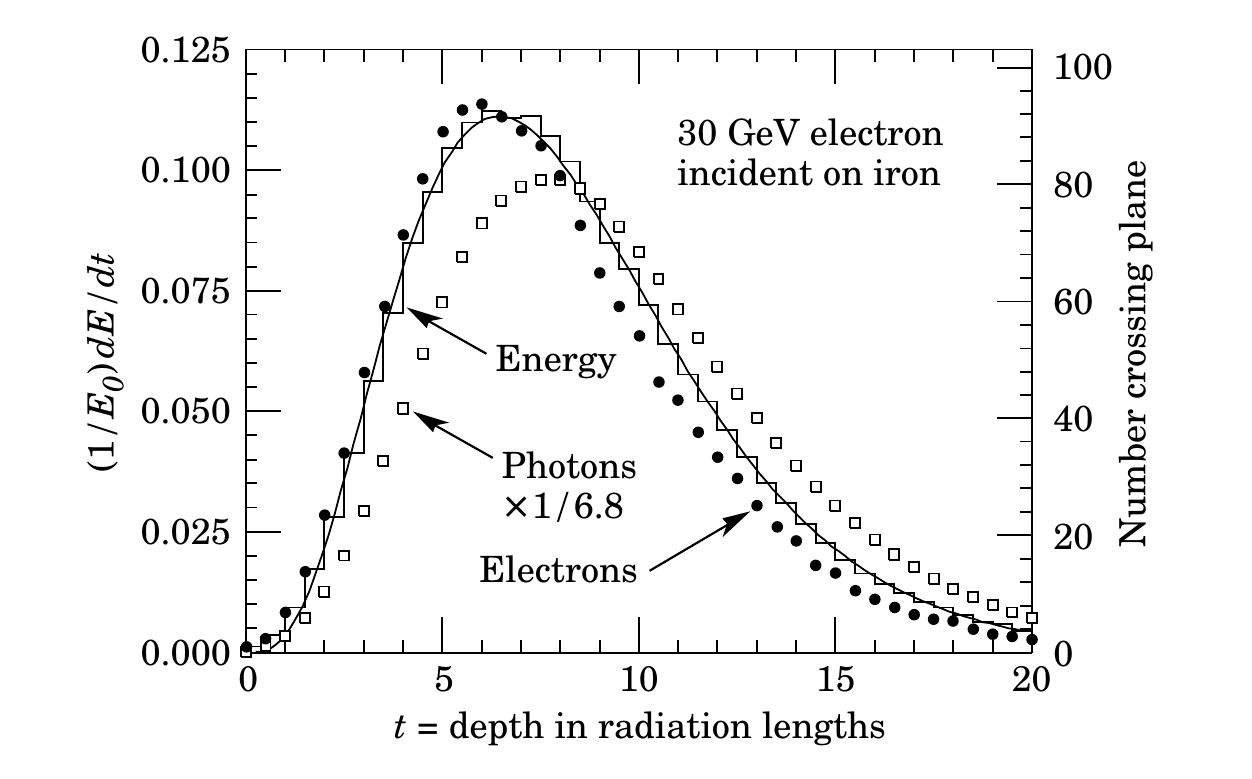
\includegraphics[width=4.0in]{e30fe.png}
  \end{center}
\end{figure}

\noindent
To understand how the shower development depends on energy, make
this plot for $E=1$ GeV and $E=10$ GeV electrons and compare
the distance at which the maximum occurs. 
In order to keep the statistical
uncertainties small, generate 1000 events at each energy.
\newpage
You will need to make a 
number of simplifying assumptions in your model: 
\begin{itemize}
\item Describe the calorimeter as a uniform  crystal of lead tungstate, 23
cm deep.  Assume electrons hit the front face of the crystal with 
fixed energy
$E$ and normal to the surface.
\item Real EM showers develop in 3-dimensions, for this problem use a 1-dimensional
model and ignore the transverse spreading of the shower.
\item Electrons lose energy by bremsstrahlung.  The mean distance
over which a high energy electron loses all but $1/e$ of its energy is
called the radiation length $X_0$.
The bremsstrahlung spectrum of
the emitted photons is peaked at low photon energy. 
While the true bremsstrahlung process is continuous, for this problem
make the {\it unrealistic} approximation that the energy loss is a discrete process
that occurs at random positions $x$ along the electron trajectory.
In other words, the number of electrons from an intial population of
$N_0$ that survive without undergoing bremmstahlung
after a distance $x$ is assumed to be 
$$
N = N_0 e^{-x/X_0}
$$
To simplify the calculation, also make the {\it unrealistic} assumption
that whenever the bremsstahlung occurs the energy is divided equally
between the the outgoing electron and photon.
\item When charged particles travel through matter, they lose energy 
via ionization.
The distribution of energy loss per unit distance is a Landau distribution,
with a mean that depends on the particle's velocity.
Assume for this problem
that the ionization energy loss per cm is constant, with
the value for lead tungstate
taken from the PDG {\it Atomic and nuclear properties of materials}.
If a charged particle ($e^+$ or $e^-$) loses enough energy via 
ionization to stop in the crystal, then it will just
be absorbed in the material. (In the real world, charged particles
have a Bragg peak in their energy loss as they stop. We will ignore
that effect here).
\item  Photons lose energy via Compton scattering, photo-nuclear 
interactions and pair production.  Assume for this problem
that pair production is
the only process that matters and that the probability of pair
production occuring distance between $x$  and $x+dx$ is
$$dP = \frac{dx}{9/7 X_0}$$
Also
{\it unrealistically} assume that the $e^+$ and $e^-$  produced 
always share the
energy of the photon equally.  Make the approximation that  the electron is massless.\\
\end{itemize}
In doing this problems, you will need to know certain physical constants (particle lifetimes,
radiation lengths of specific materials, etc).  You can find everything
you need on the Particle Data Group (PDG) web site:
  http://www-pdg.lbl.gov/
\end{document}
